\documentclass[a4paper,14pt]{extarticle}

\usepackage[utf8]{inputenc}
\usepackage[russian]{babel}
\usepackage{graphicx}
\usepackage[top=0.8in, bottom=0.8in, left=0.8in, right=0.8in]{geometry}
\usepackage{pgfplots}
\usepackage{amsmath}
\usepackage{setspace}
\usepackage{titlesec}
\usepackage{float}
\usepackage{chngcntr}
\usepackage{pgfplots}
\usepackage{amsfonts}
\usepackage{pgfplotstable}
\usepackage{multirow}
\usepackage{karnaugh-map}
\usepackage{tikz,xcolor}
\usepackage{listings}
\usepackage{indentfirst}

\lstset{ %
extendedchars=\true,
keepspaces=true,
%language=no, % choose the language of the code
basicstyle=\footnotesize, % the size of the fonts that are used for the code
numbers=left, % where to put the line-numbers
numberstyle=\footnotesize, % the size of the fonts that are used for the line-numbers
stepnumber=1, % the step between two line-numbers. If it is 1 each line will be numbered
numbersep=10pt, % how far the line-numbers are from the code
backgroundcolor=\color{white}, % choose the background color. You must add \usepackage{color}
showspaces=false, % show spaces adding particular underscores
showstringspaces=false, % underline spaces within strings
showtabs=false, % show tabs within strings adding particular underscores
frame=single, % adds a frame around the code
tabsize=4, % sets default tabsize to 2 spaces
captionpos=b, % sets the caption-position to bottom
breaklines=true, % sets automatic line breaking
breakatwhitespace=false, % sets if automatic breaks should only happen at whitespace
escapeinside={\%*}{*)}, % if you want to add a comment within your code
%postbreak=\raisebox{0ex}[0ex][0ex]{\ensuremath{\color{red}\hookrightarrow\space}}
}

\titleformat{\section}[hang]
  {\bfseries}
  {}
  {0em}
  {\hspace{-0.4pt}\large \thesection\hspace{0.6em}}
  
  
\titleformat{\subsection}[hang]
  {\bfseries}
  {}
  {0em}
  {\hspace{-0.4pt}\large \thesubsection\hspace{0.6em}}

%\linespread{1.3} % полуторный интервал
%\renewcommand{\rmdefault}{ftm} % Times New Roman

\newcommand{\nx}{\overline{x}}
\newcommand{\p}{0.31}
\newcommand{\scale}{1.4}

\counterwithin{figure}{section}
\counterwithin{equation}{section}
\counterwithin{table}{section}



\begin{document}


\begin{titlepage}
\centering
Санкт-Петербургский политехнический университет Петра Великого \\
\vspace{0.15cm}
Кафедра компьютерных систем и программных технологий \\
\vspace{6.5cm}

{\centering \textbf{Отчёт по лабораторной работе} \\ 
\vspace{0.15cm}
\textbf{Дисциплина}: Транслирующие системы \\
\vspace{0.15cm}
\textbf{Тема}: Транслятор операторов $while$ языка $C$ } \\

\vspace{6.5cm}

\begin{table}[H]
\begin{tabular}{p{\textwidth}@{}r}
{Выполнил студент гр. 43501/3} \hfill {Мальцев  М.С.} \\
{Преподаватель} \hfill {Цыган В.Н.} \\
\end{tabular}
\end{table}
\vfill

{\centering Санкт-Петербург \\ 
\vspace{0.15cm}
\today}
\end{titlepage}

\section{Задание}
    Транслятор операторов $while$ языка $C$:
    
    Тип данных: int.
    
    Условное выражение: арифметическое бесскобочнрое выражение,
    т.е. операции выполняются слева на право.

    В теле цикла:
    \begin{enumerate}
        \item операторы присваивания вида $id=$ бесскобочное арифметическое выражение
        \item вложенный оператор $while$
    \end{enumerate}

    Выходной продукт:
    \begin{enumerate}
        \item текст на языке ассембера A86
        \item тетрады матрицы синтаксического дерева
    \end{enumerate}

\section{Ход работы}
    Задание выданое преподавателем было изучено и рассмотрено с точки зрения реализуемости.\\
    
    Было решено:
    \begin{itemize}
        \item   Использовать язык ассемблера для архитектуры x86. 
                В связи с тем, что эта архитектура наиболее распространена 
                и был найден удобный транслятор из языка С в язык ассембера x86.
                (\href{https://gcc.godbolt.org/}{https://gcc.godbolt.org/})

        \item   Использовать только одну переменную. Это решение было принято
                в связи с тем, что при использовании нескольких переменных,
                помимо выявления этих переменных необходимо было бы их различать,
                что повлекло бы за собой необходимость самописной структуры данных.
                К этой структуре появляются требования, такие как расширяемость.
                Что влечёт достаточно большой объем кода, который никак не связан
                с языками $lex$ и $yacc$. Учитывая указанную проблему, было решено отказаться
                от использования нескольких переменных, но со стороны части программы, которая
                отвечает за синтаксический и лексический разбор, обеспечить необходимую функциональность для
                возможности дальнейшней работы с ними.

        \item   Отказаться от использования операций типа:
        
                int a, b, c, d;

                a = b + c + 1 + d;

                Подобное решение было связано с тем, что операции, состоящие из
                нескольких переменных, во первых были невозможны из-за предыдущего пункта
                этого списка, а во вторых из-за того что после трансляции они генерируют
                достаточно сложный текст. 

                \begin{figure}[h]
                    \center{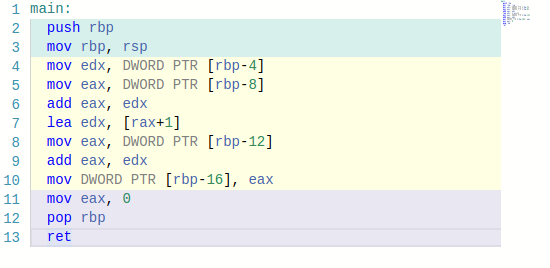
\includegraphics[scale=0.5]{img/1.png}}
                    \label{fig:image}
                \end{figure}
        
        \item   Также было решено отакзаться от вложенных циклов, в связи с тем, что
                основная сложность подобных конструкций это генерация меток, что
                не является интересной задачей, и слабо относится к языкам синтаксического и
                лексического разбора.

    \end{itemize} 

    Учитывая все перечисленные требования и нюансы была разработана программа:

    \lstinputlisting {src/c.l}
    \lstinputlisting {src/c1.y}
    \lstinputlisting {src/zz.c}

    В качестве входных данных было подано следующее:
    \lstinputlisting {src/test.in}

    В результате работы программы получили следующее:
    \lstinputlisting {src/test.out}

    Что соответствует результатам трансляции с помощью сторонней программы:
    \begin{figure}[h]
        \center{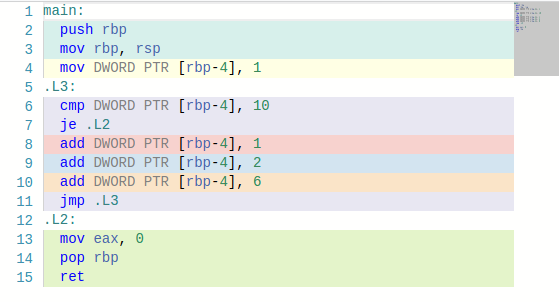
\includegraphics[scale=0.5]{img/2.png}}
        \label{fig:image}
    \end{figure}

    Следовательно, можно считать, что разработаная программа работает верно.

\section{Возможные улучшения}
    Как в случае с использованием нескольких переменных,
    так и в случае вложенных циклов $while$,
    чтобы обеспечить их поддержку необходимо  преодолеть ряд трудностей,
    которые свзяаны не с лексическим или синтаксическим разбором, а именно
    с генерацией кода на языке ассембера.
    
    В случае с вложенными циклами нужны уникальные
    значения для меток, по которым переходит программа
    во время итерации. В той реализации,
    которая предложена на данный момент метки называются одинаково.
    Что касается лексической и синтаксической обработки данных ситуаций,
    то с их стороны всё реализовано.
    
    В случае с переменными необходимо определять,
    наличие или отсутствие объявления перменной указанной в выражении -
    это можно реализовать с помощью структуры данных, которая хранит в однозначном
    соответствии имя переменной и место в памяти, где расположено
    значение.
    Причём, структура должна быть расширяющейся, так как
    мы не можем заранее предсказать сколько переменных планирует
    использовать программист.
    В этом случае проблема отсутствия реализации в итоговой программе
    заключается в том, что подобная функциональность влечёт большой
    объем кода на языке С, слабо относящийся к языкам $lex$ и $yacc$,
    изучение и работа с которыми ставятся в главные цели лабораторной работы.


\section{Вывод}
    В результате выполнения лабораторной работы был написан простейший 
    транслятор операторов $while$ языка $C$. Для написания программы
    использовались генераторы синтаксического и лексического разбора
    $yacc$ и $lex$. В ходе выполнения работы сначала было определено
    какую функциональность будет включать конечное приложение. Далее
    был разработана часть отвечающая за лексический разбор, в след за
    ней была написана часть, в задачи которой входит синтаксический разбор.
    Получившаяся программа была протестирована на различных входных данных.
    Полученные результаты соответствует тому, что было описано в задании.

    Проведенная работа позволила лучше понять принципы совместного
    использования генерторов для синтаксического и лексического разбора и
    принципы посторения трансляторов для языков программирования.
    Также в ходе выполнения лабораторной были получены навыки разработки
    приложений на основе этих языков. 


\section{Используемая литература}
    \begin{itemize}
        \item John Levine. Flex \& Bison: Text Processing Tools. — O\'{}Reilly Media, 2009
        \item Программирование лексического и синтаксического разбора на языках C, Lex и Yacc — А.В. Жуков, 2014
    \end{itemize}

\end{document}
